Вторая глава показывает расширенные конструкции. Для удобства чтения сохраняется тот же
принцип: от математического блока к табличному, затем к коду и алгоритмам. Такой порядок
помогает новичку видеть, как сложные окружения собираются в единую структуру текста ВКР.

\section{Многострочная математика и ограничения}
\subsection{Целевая функция и ограничения}
Для продвинутого примера рассматривается задача минимизации целевой функции
с набором ограничений:
\begin{align}
  \min_{x_1,x_2,x_3}\; Z &= 4x_1 + 3x_2 + 2x_3,
  \label{eq:ch2-objective} \\
  x_1 + x_2 + x_3 &= 1, \label{eq:ch2-constraint-a} \\
  2x_1 + x_2 &\ge 0.80, \label{eq:ch2-constraint-b} \\
  x_i &\ge 0,\quad i=1,2,3. \label{eq:ch2-constraint-c}
\end{align}
Формулы~\eqref{eq:ch2-objective}--\eqref{eq:ch2-constraint-c} используются как единый
связанный блок, где каждая строка имеет отдельную ссылку.

\subsection{Рекуррентная модель и режимы}
Дополнительная рекуррентная модель записывается как
\begin{gather}
  F_0 = 1,\quad F_1 = 1, \label{eq:ch2-rec-a} \\
  F_n = F_{n-1} + F_{n-2},\quad n \ge 2. \label{eq:ch2-rec-b}
\end{gather}

Режим вычисления выбирается по условию:
\begin{equation}
  \operatorname{Mode}(u)=
  \begin{cases}
    \text{offline}, & u < 0.40, \\
    \text{hybrid}, & 0.40 \le u < 0.75, \\
    \text{online}, & u \ge 0.75.
  \end{cases}
  \label{eq:ch2-mode}
\end{equation}

\section{Демонстрация длинной таблицы}
\subsection{Реестр контрольных прогонов}
Длинная таблица~\ref{tab:ch2-long} иллюстрирует работу `longtable` при переносе
на несколько страниц и аккуратное выравнивание чисел:
\begin{longtable}{@{}clS[table-format=2.2]S[table-format=1.2]@{}}
  \caption{Реестр контрольных прогонов по этапам проекта}\label{tab:ch2-long} \\
  \toprule
  № & Этап & {Длительность, ч} & {Индекс качества} \\
  \midrule
  \endfirsthead
  \caption[]{Реестр контрольных прогонов по этапам проекта (продолжение)} \\
  \toprule
  № & Этап & {Длительность, ч} & {Индекс качества} \\
  \midrule
  \endhead
  \midrule
  \multicolumn{4}{r}{Продолжение на следующей странице} \\
  \endfoot
  \bottomrule
  \endlastfoot
  1  & Сбор требований                     & 12.50 & 0.78 \\
  2  & Проектирование структуры            & 10.00 & 0.81 \\
  3  & Подготовка титульного листа         & 5.50  & 0.88 \\
  4  & Настройка шрифтов                   & 6.25  & 0.92 \\
  5  & Разметка формул                     & 8.75  & 0.85 \\
  6  & Разметка рисунков                   & 7.00  & 0.86 \\
  7  & Разметка таблиц                     & 9.25  & 0.87 \\
  8  & Реализация листингов                & 6.50  & 0.90 \\
  9  & Реализация алгоритмов               & 7.40  & 0.91 \\
  10 & Настройка перекрестных ссылок       & 4.80  & 0.95 \\
  11 & Тестирование пайплайна              & 6.10  & 0.96 \\
  12 & Корректировка методических пояснений& 5.70  & 0.89 \\
  13 & Подготовка приложений               & 7.90  & 0.90 \\
  14 & Финальный прогон сборки             & 3.60  & 0.98 \\
  15 & Предзащитная валидация              & 4.20  & 0.97 \\
\end{longtable}

\subsection{Архитектурная иллюстрация}
Дополнительная архитектурная иллюстрация приведена на рисунке~\ref{fig:ch2-cache};
она показывает роль кэш-уровня в снижении латентности запроса.
Источник диаграммы: открытый репозиторий системного проектирования~\cite{sdp-cache}.
\begin{figure}[tbp]
  \centering
  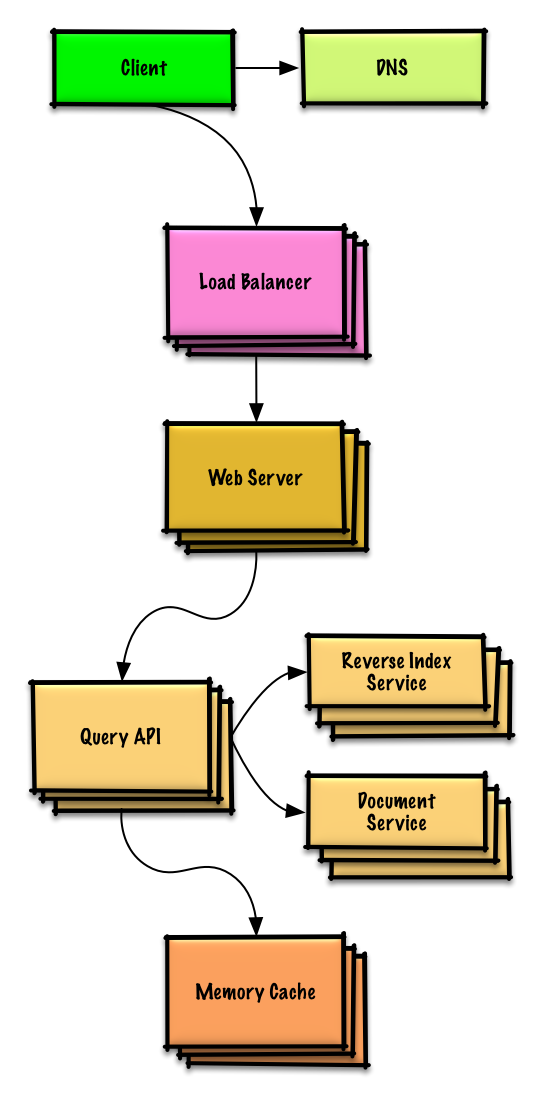
\includegraphics[width=0.64\linewidth]{assets/images/fig-04-query-cache-architecture.png}
  \caption{Архитектура кэширования запросов в распределенном сервисе}
  \label{fig:ch2-cache}
\end{figure}

\section{Демонстрация листингов}
\subsection{Python-листинг проверки структуры}
Листинг~\ref{lst:ch2-validator} показывает рабочий пример кода, который
обходит каталог контента и проверяет наличие ожидаемых файлов:
\begin{lstlisting}[caption={Скрипт валидации структуры контента},label={lst:ch2-validator}]
from pathlib import Path

CONTENT_FILES = [
    "01-introduction.tex",
    "02-chapter-1.tex",
    "03-chapter-2.tex",
    "04-conclusion.tex",
]

root = Path("content")
missing = [name for name in CONTENT_FILES if not (root / name).exists()]

if missing:
    print("Missing files:", ", ".join(missing))
else:
    print("Content structure is valid.")
\end{lstlisting}

\subsection{Bash-фрагмент сборочного сценария}
Для демонстрации конфигурационного фрагмента используется листинг~\ref{lst:ch2-make-target}:
\begin{lstlisting}[language=bash,caption={Пример цели Makefile для сборки},label={lst:ch2-make-target}]
build:
	latexmk -pdf -lualatex main.tex
\end{lstlisting}

\subsection{LaTeX-листинги шаблонов}
Листинги LaTeX оформляются с локальным указанием языка, чтобы новичкам было проще
сопоставлять окружения, команды и метки:
\begin{lstlisting}[language={[LaTeX]TeX},texcsstyle=*\color{lstKeyword},alsoletter={\\},morekeywords={begin,end,chapter,section,subsection,label,ref,eqref,caption,includegraphics},caption={Шаблон нумеруемой формулы с меткой},label={lst:ch2-latex-equation}]
\begin{equation}
  S = \sum_{i=1}^{n} w_i x_i,
  \label{eq:weighted-score}
\end{equation}
\end{lstlisting}

\begin{lstlisting}[language={[LaTeX]TeX},texcsstyle=*\color{lstKeyword},alsoletter={\\},morekeywords={begin,end,chapter,section,subsection,label,ref,eqref,caption,includegraphics},caption={Шаблон рисунка с подписью и ссылкой},label={lst:ch2-latex-figure}]
\begin{figure}[tbp]
  \centering
  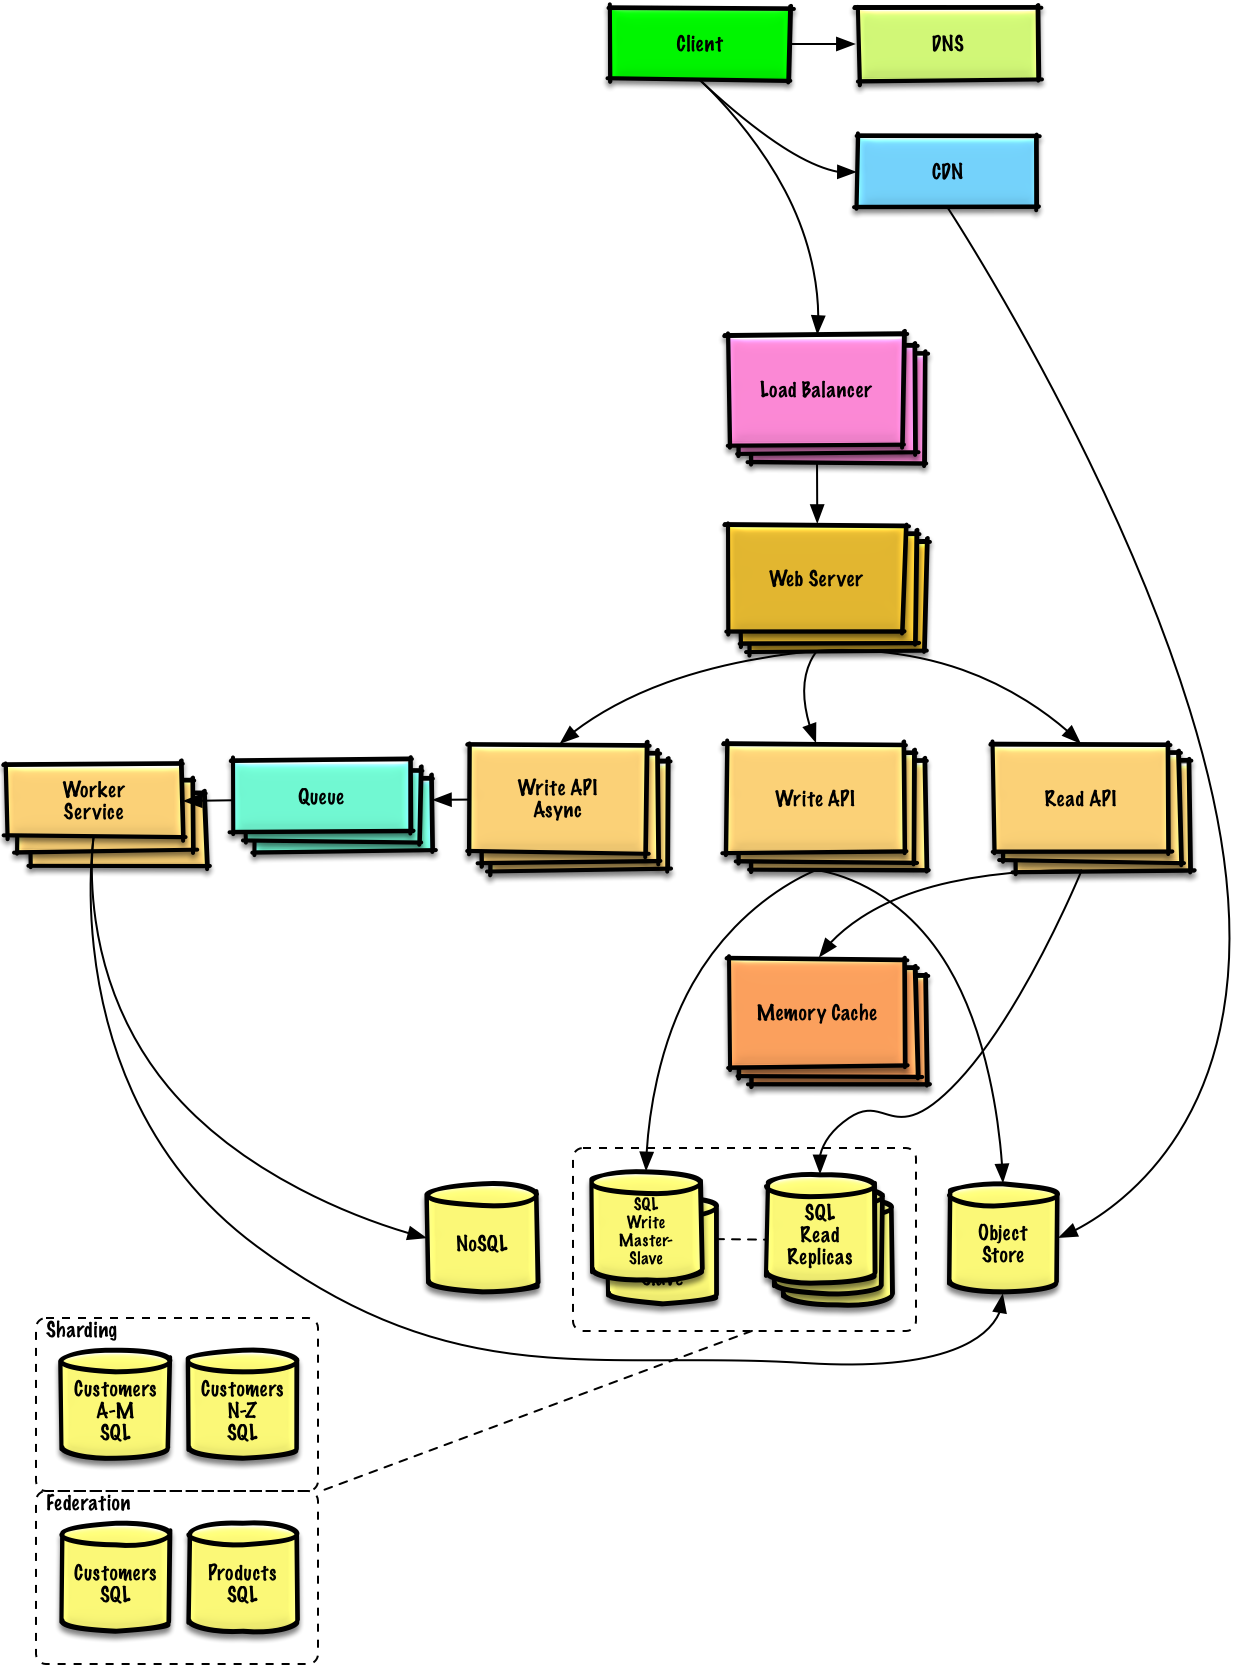
\includegraphics[width=0.8\linewidth]{assets/images/fig-05-aws-scaling-architecture.png}
  \caption{Схема масштабирования сервиса в облачной среде}
  \label{fig:scaling-demo}
\end{figure}
\end{lstlisting}

\section{Демонстрация алгоритмов}
\subsection{Псевдокод формирования отчета}
Алгоритм~\ref{alg:ch2-report} демонстрирует псевдокод построения отчета качества:
\begin{algorithm}[tbp]
  \caption{Формирование отчета контроля сборки}
  \label{alg:ch2-report}
  \begin{algorithmic}[1]
    \Require Массив `checks`, содержащий статусы проверок
    \Ensure Текстовый отчет `report`
    \State `passed` $\gets$ 0
    \State `report` $\gets$ пустой список
    \ForAll{элемент `check` в `checks`}
      \If{`check.status` = ``ok''}
        \State `passed` $\gets$ `passed` + 1
        \State добавить строку ``OK: check.name'' в `report`
      \Else
        \State добавить строку ``FAIL: check.name'' в `report`
      \EndIf
    \EndFor
    \State добавить итог ``passed / |checks|'' в `report`
    \State \Return `report`
  \end{algorithmic}
\end{algorithm}

\section{Композитный кейс 2: полный advanced-блок}
\subsection{Интеграция сложных элементов}
Для демонстрации сквозного сценария в одной связке используются:
формула оптимизации~\eqref{eq:ch2-objective}, длинная таблица~\ref{tab:ch2-long},
листинг валидации~\ref{lst:ch2-validator}, алгоритм~\ref{alg:ch2-report}
и визуальные схемы~\ref{fig:ch1-subfig},~\ref{fig:ch2-cache}.

\subsection{Практические ориентиры по оформлению}
Кейс показывает, что даже при усложнении синтаксиса документ остается управляемым:
каждый элемент имеет устойчивую ссылку, подпись и воспроизводимую сборку.
Для практики рекомендуется опираться на официальные справочники пакетов
`listings`, `algorithmicx` и `siunitx`~\cite{listings-doc,algpseudocode-doc,siunitx-doc},
а также на общую методологию literate programming~\cite{knuth1984}
и примеры архитектурных схем открытого сообщества~\cite{sdp-repo,sdp-aws}.
